
\documentclass[border=10pt]{standalone}
\usepackage{pgfplots}
\pgfplotsset{compat=1.18}
\begin{document}
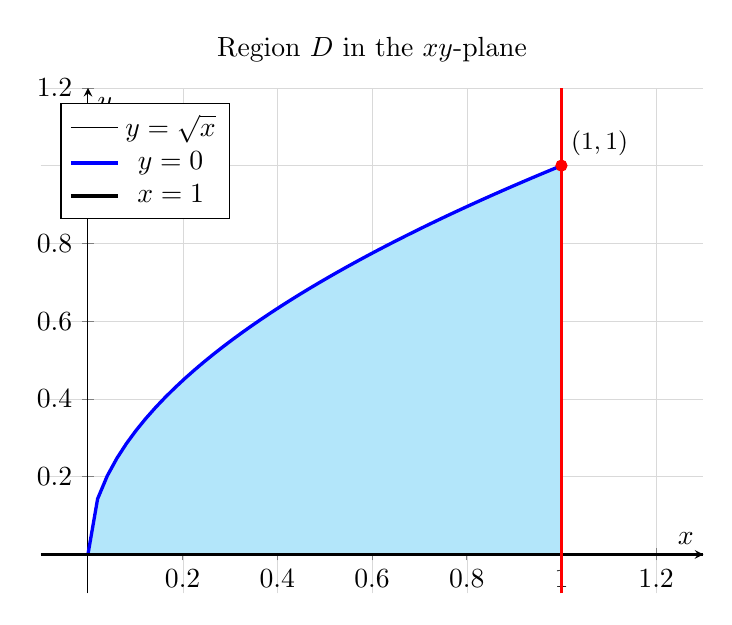
\begin{tikzpicture}
\begin{axis}[
    xlabel={$x$},
    ylabel={$y$},
    title={Region $D$ in the $xy$-plane},
    xmin=-0.1, xmax=1.3,
    ymin=-0.1, ymax=1.2,
    grid=both,
    grid style={line width=.1pt, draw=gray!30},
    axis lines=middle,
    legend pos=north west,
    samples=100,
    width=10cm, height=8cm
]
% Filled region
\addplot[fill=cyan!30, draw=none, domain=0:1, samples=50] {sqrt(x)} \closedcycle;
% Curves
\addplot[blue, very thick, domain=0:1, samples=50] {sqrt(x)};
\addlegendentry{$y=\sqrt{x}$}
\addplot[black, very thick, domain=-0.1:1.3] {0};
\addlegendentry{$y=0$}
\addplot[red, very thick, domain=-0.1:1.2] (1, x);
\addlegendentry{$x=1$}
% Vertex
\addplot[only marks, mark=*, mark size=2pt, color=red] coordinates {(1,1)};
\node[above right] at (axis cs:1,1) {\small $(1,1)$};
\end{axis}
\end{tikzpicture}
\end{document}
